\section{AutoPhase Framework for Automatic Phase Ordering} 
\label{sec:framework}

We leverage an existing open-source HLS framework called LegUp~\cite{canis2013legup} that compiles a C program into a hardware RTL design. 
In \cite{huang2013effect}, an approach is devised to quickly determine the number of hardware execution cycles without requiring time-consuming logic simulation.
We develop our RL simulator environment based on the existing harness provided by LegUp and validate our final results by going through the time-consuming logic simulation. AutoPhase takes a program (or multiple programs) and intelligently explores the space of possible passes to figure out an optimal pass sequence to apply. Table~\ref{tab:passes} lists all the passes used in AutoPhase. The workflow of AutoPhase is illustrated in Figure~\ref{fig:framework}.


\subsection{HLS Compiler}
AutoPhase takes a set of programs as input and compiles them 
%front-end of the LLVM compiler. LLVM represents programs 
to a hardware-independent intermediate representation (IR) using the Clang front-end of the LLVM compiler. Optimization and analysis passes act as transformations on the IR, taking a program as input and emitting a new IR as output. The HLS tool LegUp is invoked after the compiler optimization as a back-end pass, which transforms LLVM IR into hardware modules.
%The compute logic is turned into a hardware datapath and the control logic is turned into a hardware FSM respectively by the HLS tool. 
%Its SDC-based scheduler \cite{cong2006efficient} operates at the basic block level to exploit the instruction-level parallelism. 
\begin{figure}[t!]
    \centering
    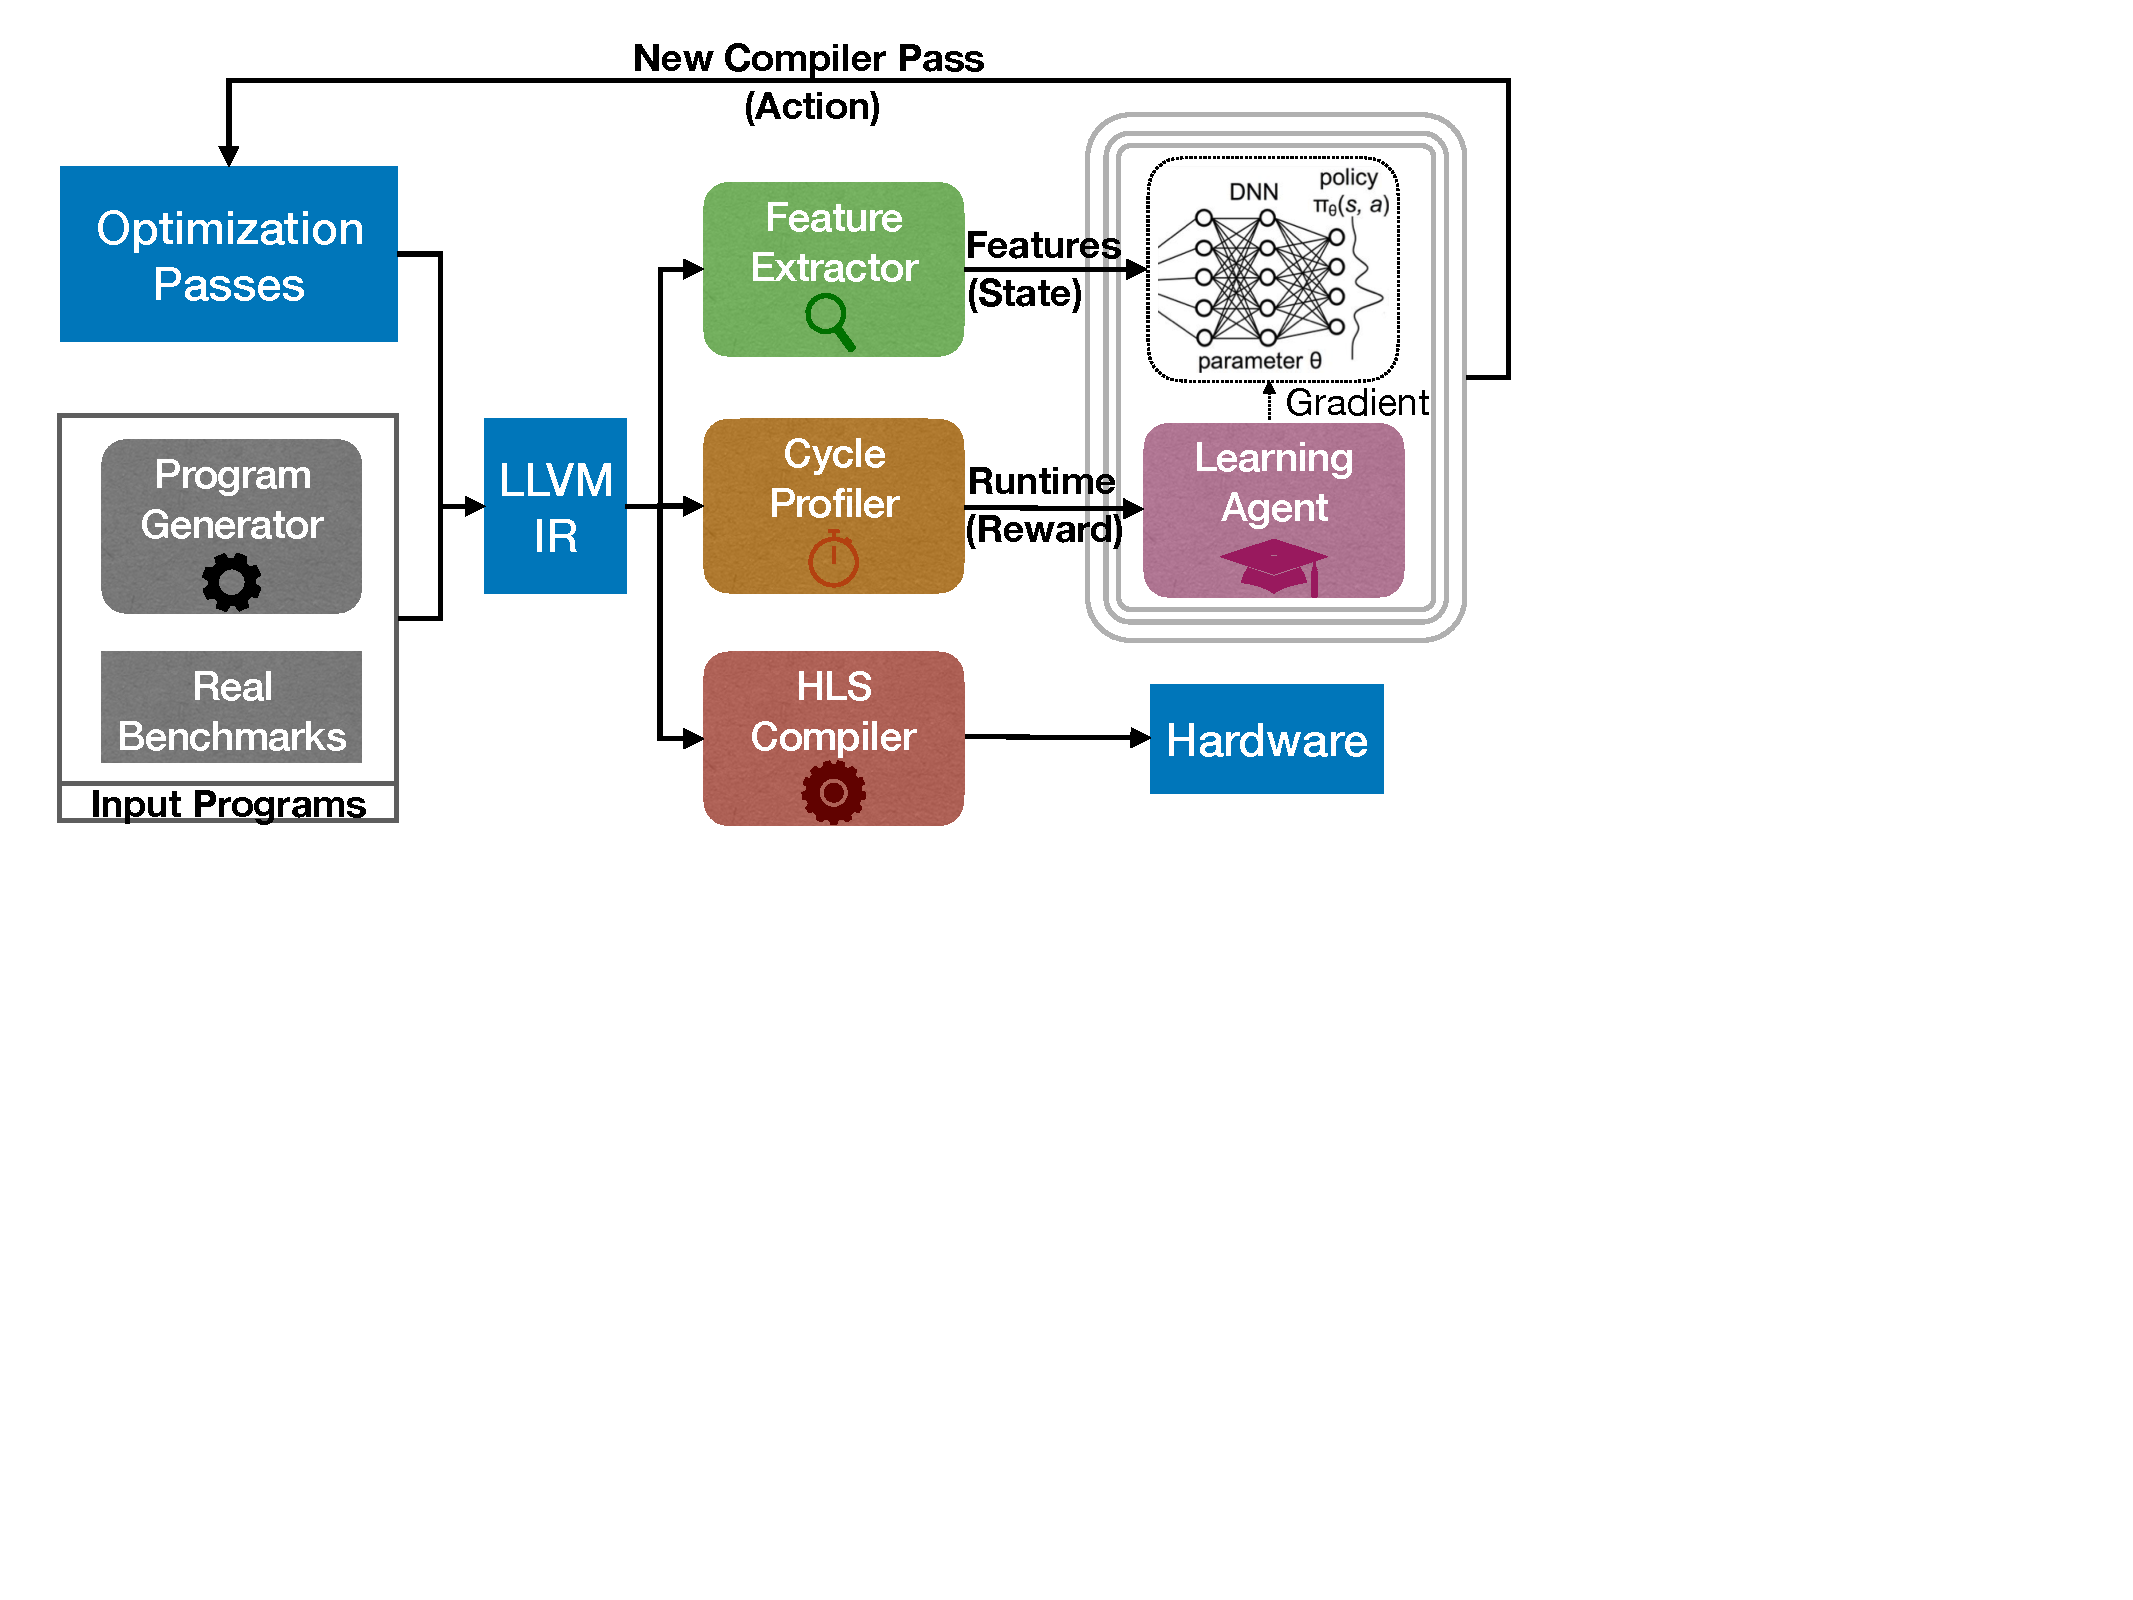
\includegraphics[width=0.48\textwidth]{Figures/Framework.pdf}
    \caption{The block diagram of AutoPhase. The input programs are compiled to an LLVM IR using Clang/LLVM. The feature extractor and clock-cycle profiler are used to generate the input features (state) and the runtime improvement (reward), respectively from the IR. The input features and runtime improvement are fed to the deep RL agent as in input data to train on. The RL agent predicts the next best optimization passes to apply. After convergence, the HLS compiler is used to compile the LLVM IR to hardware RTL.}
    \label{fig:framework}
    \vspace{-0.5cm}
\end{figure}
\subsection{Clock-cycle Profiler}
Once the hardware RTL is generated, one could run a hardware simulation to gather the cycle count results of the synthesized circuit. This process is quite time-consuming, hindering RL and all other optimization approaches. Therefore, we approximate cycle count using the profiler in LegUp~\cite{huang2013effect}, which leverages the software traces and runs $20\times$ faster than hardware simulation. 
In LegUp, the frequency of the generated circuits is set as a compiler constraint that directs the HLS scheduling algorithm. In other words, HLS tool will always try to generate hardware that can run at a certain frequency. In our experiment setting, without loss of generality, we set the target frequency of all generated hardware to 200MHz. We experimented with lower frequencies too; the improvements were similar but the cycle counts the different algorithms achieved were better as more logic could be fitted in a single cycle. 
%The profiler first runs the software program to gather information on the number of times each basic block is executed, then multiplies it with the clock cycle time of the basic block determined by the HLS scheduler to produce the total clock cycle time of the circuit. This software approach is $20\times$ faster than hardware simulation, which significantly reduces the runtime bottleneck of the deep reinforcement learning algorithm. 

\subsection{IR Feature Extractor}
Wang \textit{et al.}~\cite{wang2018} proposed to convert a program into an observation by extracting all the features from the program. Similarly, in addition to the LegUp backend tools, we developed analysis passes to extract 56 static features from the program, such as the number of basic blocks, branches, and instructions of various types. 
%Each individual feature is insufficient to guide the machine learning algorithm.
We use these features as partially observable states for the RL learning and hope the neural network can capture the correlation of certain combinations of these features and certain optimizations. Table \ref{tab:tab1} lists all the features used.
%All the features we gather are listed in Table~\ref{tab:tab1} in the appendix. 
%The framework takes a program or multiple ones and compiles them using the LLVM compiler, which was modified to output the program features. The HLS toolchain is used to extract the number of cycles that are used as the cost function to the RL architecture to find the optimal passes. 

\subsection{Random Program Generator}
As a data-driven approach, RL generalizes better if we train the agent on more programs.
However, there are a limited number of open-source HLS examples online. Therefore, we expand our training set by automatically generating synthetic HLS benchmarks. We first generate standard C programs using CSmith~\cite{yang2011csmith}, a random C program generator, which is originally designed to generate test cases for finding compiler bugs. Then, we develop scripts to filter out programs that take more than five minutes to run on CPU or fail the HLS compilation. 

\subsection{Overall Flow of AutoPhase}
We integrate the compilation utilities into a simulation environment in Python with APIs similar to an OpenAI gym~\cite{brockman2016openai}.
%The programs are compiled , features and cycles are extracted from the IR and HLS toolchain respectively, and are afterwards fed to the RL network to learn the optimal passes. 
%Our environment takes an input program and returns the program feature vectors and the total number of clock cycles. We consider two types of features as the state for the RL: the current program IR and the sequence of passes that have been applied. 
The overall flow works as follows:
\begin{enumerate}
\itemsep 0em 
\item The input program is compiled into LLVM IR using the Clang/LLVM. 
\item The IR Feature Extractor is run to extract salient program features. 
\item LegUp compiles the LLVM IR into hardware RTL.
\item The Clock-cycle Profiler estimates a clock-cycle count for the generated circuit. 
\item The RL agent takes the program features or the histogram of previously applied passes and the improvement in clock-cycle count as input data to train on. 
%are fed into the RL agent to derive a good LLVM optimization sequence.
%In RL specifically, the clock-cycle time is used for reward calculation, and the program features are used as partially observable states for the RL agents. 
\item The RL agent predicts the next best optimization passes to apply. 
%In iterative methods (\textit{i.e.}, greedy algorithm, genetic algorithm, and RL), the algorithm then predicts the next best action to take. In RL, the action would be the next optimization to apply to the end of an existing sequence of passes. In a modified greedy algorithm, the next action could be the next best place to insert the optimization pass.
\item New LLVM IR is generated after the new optimization sequence is applied. 
\item The machine learning algorithm iterates through steps (2)--(7) until convergence.
\end{enumerate}
Note that AutoPhase uses the LLVM compiler and the passes used are listed in Table~\ref{tab:tab1}. However, adding support for any compiler or optimization passes in AutoPhase is very easy and straightforward. The action and state definitions must be specified again. 
\begin{table*}[!t]
\caption{LLVM Transform Passes.}
\scriptsize
\centering
\begin{tabular}{ccccccccccc}
\hline
0 & 1 & 2 & 3 & 4 & 5 & 6 & 7 & 8 & 9 & 10 \\
-correlated-propagation & -scalarrepl & -lowerinvoke & -strip & -strip-nondebug & -sccp & -globalopt & -gvn & -jump-threading & -globaldce & -loop-unswitch \\
\end{tabular}
\begin{tabular}{ccccccccccc}
\hline
11 & 12 & 13 & 14 & 15 & 16 & 17 & 18 & 19 & 20 & 21 \\
-scalarrepl-ssa & -loop-reduce & -break-crit-edges & -loop-deletion & -reassociate & -lcssa & -codegenprepare & -memcpyopt & -functionattrs & -loop-idiom & -lowerswitch \\
\end{tabular}
\begin{tabular}{cccccccccccc}
\hline
22 & 23 & 24 & 25 & 26 & 27 & 28 & 29 & 30 & 31 & 32 & 33 \\
-constmerge & -loop-rotate & -partial-inliner & -inline & -early-cse & -indvars & -adce & -loop-simplify & -instcombine & -simplifycfg & -dse & -loop-unroll \\
\end{tabular}
\begin{tabular}{cccccccccccc}
\hline
34 & 35 & 36 & 37 & 38 & 39 & 40 & 41 & 42 & 43 & 44 & 45 \\
-lower-expect & -tailcallelim & -licm & -sink & -mem2reg & -prune-eh & -functionattrs & -ipsccp & -deadargelim & -sroa & -loweratomic & -terminate \\
\hline
\end{tabular}
\label{tab:passes}

\end{table*}
\begin{table*}[!t]
\scriptsize
\centering
\caption{Program Features.}
\begin{tabular}{
|c|c|c|c|}
\hline 0&
Number of BB where total args for phi nodes \textgreater 5 & 28&  Number of And insts \\ \hline 1&
Number of BB where total args for phi nodes is {[}1,5{]} & 29&  Number of BB's with instructions between {[}15,500{]} \\ \hline 2&
Number of BB's with 1 predecessor & 30&  Number of BB's with less than 15 instructions \\ \hline 3&
Number of BB's with 1 predecessor and 1 successor & 31&  Number of BitCast insts \\ \hline 4&
Number of BB's with 1 predecessor and 2 successors & 32&  Number of Br insts \\ \hline 5&
Number of BB's with 1 successor & 33&  Number of Call insts \\ \hline 6&
Number of BB's with 2 predecessors & 34&  Number of GetElementPtr insts \\ \hline 7&
Number of BB's with 2 predecessors and 1 successor & 35&  Number of ICmp insts \\ \hline 8&
Number of BB's with 2 predecessors and successors & 36&  Number of LShr insts \\ \hline 9&
Number of BB's with 2 successors & 37&  Number of Load insts \\ \hline 10&
Number of BB's with \textgreater{}2 predecessors & 38&  Number of Mul insts \\ \hline 11&
Number of BB's with Phi node \# in range (0,3{]} & 39&  Number of Or insts \\ \hline 12&
Number of BB's with more than 3 Phi nodes & 40&  Number of PHI insts \\ \hline 13&
Number of BB's with no Phi nodes & 41&  Number of Ret insts \\ \hline 14&
Number of Phi-nodes at beginning of BB & 42&  Number of SExt insts \\ \hline 15&
Number of branches & 43&  Number of Select insts \\ \hline 16&
Number of calls that return an int & 44&  Number of Shl insts \\ \hline 17&
Number of critical edges & 45&  Number of Store insts \\ \hline 18&
Number of edges & 46&  Number of Sub insts \\ \hline 19&
Number of occurrences of 32-bit integer constants & 47&  Number of Trunc insts \\ \hline 20&
Number of occurrences of 64-bit integer constants & 48&  Number of Xor insts \\ \hline 21&
Number of occurrences of constant 0 & 49&  Number of ZExt insts \\ \hline 22&
Number of occurrences of constant 1 & 50&  Number of basic blocks \\ \hline 23&
Number of unconditional branches & 51&  Number of instructions (of all types) \\ \hline 24&
Number of Binary operations with a constant operand & 52&  Number of memory instructions \\ \hline 25&
Number of AShr insts & 53&  Number of non-external functions \\ \hline 26&
Number of Add insts & 54&  Total arguments to Phi nodes \\ \hline 27&
Number of Alloca insts & 55&  Number of Unary operations \\ \hline
\end{tabular}
\label{tab:tab1}
\vspace{-0.1cm}
\end{table*}


